
% Desenvolvido por: Prof. Dr. David Buzatto
% Adaptado por: Prof. Dr. Fernando Carvalho
%
% Baseado na documentação do abntex2 e nos modelos em
% Microsoft Word propostos pela Profa. Dra. Rosana F. L. Rodrigues
% e pela bibliotecária M.Sc. Maria Carolina Gonçalves do câmpus
% São João da Boa Vista do IFSP.
%
% Versão 1.5
% Data: 03/09/2018


\documentclass[
	% -- opções da classe memoir --
	12pt,				% tamanho da fonte
	openany,			% capítulos começam em pág ímpar openright (insere página vazia caso preciso)
	oneside,			% para impressão em verso e anverso (twoside). Oposto a oneside 
	a4paper,			% tamanho do papel. 
	normalfigtabnum,
	pnumromarab,
	% -- opções da classe abntex2 --
	chapter=TITLE,		% títulos de capítulos convertidos em letras maiúsculas
	section=TITLE,		% títulos de seções convertidos em letras maiúsculas
	%subsection=TITLE,	% títulos de subseções convertidos em letras maiúsculas
	%subsubsection=TITLE,% títulos de subsubseções convertidos em letras maiúsculas
	% -- opções do pacote babel --
	english,			% idioma adicional para hifenização
	french,				% idioma adicional para hifenização
	spanish,			% idioma adicional para hifenização
	brazil,				% o último idioma é o principal do documento
]{abntex2}

% \usepackage{blindtext, showframe}

% \usepackage[a4paper,showframe,
% top    = 2.75cm,
% bottom = 2.50cm,
% left   = 3.00cm,
% right  = 2.50cm]{geometry}


%%%%%%%%%%%%%%%%%%%%%%%%%%%%%%%%%%%%%%%%%%%%%%%%%%%%%%%%%%%%


\newenvironment{conditions}[1][onde:]
  {\noindent
	#1
	
	\indent
	\begin{tabular}[t]{>{$}l<{$} @{${} \> \> {}$} l}}
	{\end{tabular}\\[\belowdisplayskip]}


% --- Controla a geração de listas de siglas, símbolos e glossário
% \RequirePackage[style=long]{glossaries}
% ,long,numberlist


\usepackage[acronyms,symbols]{glossaries}
\setacronymstyle{long-short}

% \makenoidxglossaries


%Definição das listas de glossários e parâmertos para compilação.
%-------------------------------------------------------
\newglossary{verbetes}{verbetes}{vrl}{verbetes}
\newglossary{siglas}{siglas}{sgl}{siglas}
\newglossary{simbolos}{simbolos}{sbl}{simbolos}


%Definição dos comandos para exibição das listas individuais.
%-----------------------------------------------------------
\newcommand{\listarsiglas}{\printglossary[type=siglas, title=\listadesiglasname, nonumberlist=true]}
\newcommand{\listarsimbolos}{\printglossary[type=simbolos, title=\listadesimbolosname, nonumberlist=true]}
\newcommand{\listarverbetes}{\printglossary[type=verbetes]}

%Definição dos Comandos para inclusão no texto das siglas.

\newcommand{\verbete}[3]{
	\newglossaryentry{glossary}{name=#1, description={#2}, plural={#3}, type=verbetes}
	\gls{#1}
}

\newcommand{\sigla}[2]{
	\newacronym[type=siglas]{#1}{#1}{#2}
	\gls{#1}
}

\newcommand{\simbolo}[3]{
	\newglossaryentry{#1}{type=simbolos, name=#3, text=#3, description=#2,symbol=#3, sort=def}
	\gls{#1}
}

%%%%%%%%%%%%%%%%%%%%%%%%%%%%%%%%%%%%%%%%%%%%%%%%%%%%%%%%%%%%

\RequirePackage{bookmark}   			



% ---------------------------------------------------------------------------------
%                                   PACOTES
% ---------------------------------------------------------------------------------


% ---
% Pacotes básicos 
% ---

\usepackage{cmap}
\usepackage{lmodern}

\usepackage{amsmath}
\usepackage{latexsym}
\usepackage{amsfonts}
\usepackage[normalem]{ulem}
\usepackage{array}
\usepackage{amssymb}
\usepackage{graphicx}

% \usepackage[backend=bibtex,
% style=authoryear,
% natbib=true,
% sorting=none,
% isbn=false,
% doi=false,
% url=false,

\usepackage{subfig}
\usepackage{wrapfig}
\usepackage{wasysym}
\usepackage{enumitem}
\usepackage{adjustbox}
\usepackage{ragged2e}
\usepackage[svgnames,table]{xcolor}
\usepackage{tikz}
\usetikzlibrary{intersections}
\usetikzlibrary{shapes,arrows,chains}
\tikzstyle{line}=[draw] % here
\usepackage{longtable}
\usepackage{changepage}
\usepackage{setspace}
\usepackage{hhline}
\usepackage{multicol}
\usepackage{tabto}
\usepackage{multirow}
\usepackage{makecell}
\usepackage{fancyhdr}



\usepackage{lmodern}			% Usa a fonte Latin Modern			
\usepackage[T1]{fontenc}		% Selecao de codigos de fonte.
\usepackage[utf8]{inputenc}		% Codificacao do documento (conversão automática dos acentos)
\usepackage{lastpage}			% Usado pela Ficha catalográfica
\usepackage{indentfirst}		% Indenta o primeiro parágrafo de cada seção.
\usepackage{xcolor,colortbl}	% Controle das cores
\usepackage{graphicx}			% Inclusão de gráficos
\usepackage{microtype} 			% para melhorias de justificação
\usepackage{hyperref}
\usepackage{subfig}
\usepackage{epigraph}
\usepackage{url}
\usepackage{placeins}
\usepackage{multirow}
\usepackage[figuresright]{rotating}
\usepackage{chemfig}
\usepackage{amsmath}
\usepackage{amssymb}
\usepackage{enumitem}
\usepackage{bigints}
\usepackage{listings}
\usepackage{etoolbox}
\usepackage[final]{pdfpages}
\usepackage{bigstrut}
\usepackage{makeidx}
\usepackage{float}

% ---



% ---
% Pacotes adicionais, usados apenas no âmbito do Modelo Canônico do abnteX2
% ---
\usepackage{lipsum}				% para geração de dummy text
% ---

% ---
% Pacotes de citações
% ---
\usepackage[brazilian,hyperpageref]{backref}	 % Paginas com as citações na bibl
% \usepackage[alf,abnt-emphasize=bf]{abntex2cite}  % Citações padrão ABNT
\usepackage[alf]{abntex2cite}  % Citações padrão ABNT


% ---------------------------------------------------------------------------------
%                          CONFIGURAÇÕES DOS PACOTES
% ---------------------------------------------------------------------------------

% ---
% Configurações do pacote backref
%
% Para desativar, tire o comentário de \begin{comment} e \end{comment} 
% das próximas linhas e comente a linha \usepackage[brazilian,hyperpageref]{backref}
% acima.
% ---

% \newcommand{\imprimirdata}{\data}


%\begin{comment}
% ---
% Configurações do pacote backref
% Usado sem a opção hyperpageref de backref
\renewcommand{\backrefpagesname}{Citado na(s) página(s):~}
% Texto padrão antes do número das páginas
\renewcommand{\backref}{}
% Define os textos da citação
\renewcommand*{\backrefalt}[4]{
	\ifcase #1 %
	Nenhuma citação no texto.%
	\or
	Citado na página #2.%
	\else
	Citado #1 vezes nas páginas #2.%
	\fi}%
% ---
%\end{comment}


% listagens
\definecolor{corComentario}{RGB}{150,150,150}
\definecolor{corString}{RGB}{206,123,0}
\definecolor{corPalavraChave}{RGB}{0,0,230}

\lstset{
	numbers=left,
	stepnumber=1,
	firstnumber=1,
	numberstyle=\footnotesize,
	extendedchars=true,
	breaklines=true,
	lineskip=0pt,
	frame=tb,
	basicstyle=\ttfamily\footnotesize,
	showstringspaces=false,
	stringstyle=\color{corString},
	commentstyle=\color{corComentario},
	keywordstyle=\color{corPalavraChave}
}

\newcommand{\graficoname}{Gráfico}
\newcommand{\graficorefname}{Gráfico}
\newcommand{\listofgraficosname}{Lista de gráficos}





% \newcolumntype{Y}{>{\centering\arraybackslash}X}

\newcommand{\ano}[1]{\def \oano {#1}}
\newcommand{\imprimirano}{\oano}

\newcommand{\mes}[1]{\def \omes {#1}}
\newcommand{\imprimirmes}{\omes}

\newcommand{\dia}[1]{\def \odia {#1}}
\newcommand{\imprimirdia}{\odia}

% \newcommand{\subtitulo}[1]{\def \osubtitulo {#1}}
% \newcommand{\imprimirsubtitulo}{\osubtitulo}

\newcommand{\area}[1]{\def \aarea {#1}}
\newcommand{\imprimirarea}{\aarea}

\newcommand{\disciplina}[1]{\def \adisciplina {#1}}
\newcommand{\imprimirdisciplina}{\adisciplina}

% \renewcommand{\coorientador}[1]{\def \ocoorientador {#1}}
% \renewcommand{\imprimircoorientador}{\ocoorientador}

\newcommand{\grau}[1]{\def \ograu {#1}}
\newcommand{\imprimirgrau}{\ograu}

\newcommand{\curso}[1]{\def \ocurso {#1}}
\newcommand{\imprimircurso}{\ocurso}

\newcommand{\campus}[1]{\def \ocampus {#1}}
\newcommand{\imprimircampus}{\ocampus}

\newcommand{\instituicaoOrientador}[1]{\def \aInstituicaoOrientador {#1}}
\newcommand{\imprimirInstituicaoOrientador}{\aInstituicaoOrientador}

\newcommand{\instituicaoCoorientador}[1]{\def \aInstituicaoCoorientador {#1}}
\newcommand{\imprimirInstituicaoCoorientador}{\aInstituicaoCoorientador}

\newcommand{\instituicaoProfBancaA}[1]{\def \aInstituicaoProfBancaA {#1}}
\newcommand{\imprimirInstituicaoProfBancaA}{\aInstituicaoProfBancaA}

\newcommand{\instituicaoProfBancaB}[1]{\def \aInstituicaoProfBancaB {#1}}
\newcommand{\imprimirInstituicaoProfBancaB}{\aInstituicaoProfBancaB}

\providecommand{\imprimirProfBancaARotulo}{}
\providecommand{\imprimirProfBancaAnome}{}
\newcommand{\ProfBancaA}[2][]%
  {\renewcommand{\imprimirProfBancaARotulo}{#1}%
   \renewcommand{\imprimirProfBancaAnome}{#2}}


\providecommand{\imprimirProfBancaBRotulo}{}
\providecommand{\imprimirProfBancaBnome}{}
\newcommand{\ProfBancaB}[2][]%
  {\renewcommand{\imprimirProfBancaBRotulo}{#1}%
   \renewcommand{\imprimirProfBancaBnome}{#2}}



% Área de Concentração: \imprimirarea}
% ---


% ---
% Configurações de aparência do PDF final
% ---

% alterando o aspecto da cor azul
\definecolor{blue}{RGB}{41,5,195}

% informações do PDF
\makeatletter
\hypersetup{
	%pagebackref=true,
	pdftitle={\@title}, 
	pdfauthor={\@author},
	pdfsubject={\imprimirpreambulo},
	pdfcreator={\@author},
	pdfkeywords={Palavra chave 1}{Palavra chave 2}{Palavra chave 3}{Palavra chave n}, 
	colorlinks=true,       		% false: boxed links; true: colored links
	linkcolor=blue,          	% color of internal links
	citecolor=blue,       		% color of links to bibliography
	filecolor=black,      		% color of file links
	urlcolor=blue,
	bookmarksdepth=4
}
\makeatother
% --- 


% ---
% Comandos do autor
% ---

% comando para inserir autor e ano
\newcommand{\citeauthorandyear}[1]{\citeauthoronline{#1} (\citeyear{#1})}

% --- 
% Espaçamentos entre linhas e parágrafos 
% --- 

% O tamanho do parágrafo é dado por:
\setlength{\parindent}{1.3cm}

% Controle do espaçamento entre um parágrafo e outro:
\setlength{\parskip}{0.2cm}  % tente também \onelineskip

\glsaddall

% ---
% compila os glossários e listas
%\makeglossaries

% ---
% compila o indice
% ---
\makeindex
% ---
%---


%%%%%%%%%%%%%%%%%%%%%%%%%%%%%%%%%%%%%%%%%%%%

% para o pacote "Lst Listing"

\newcommand{\source}[1]{\caption*{Fonte: {#1}}}

% Altera o nome padrão do rótulo usado no comando \autoref{}
\renewcommand{\lstlistingname}{Código}

% Altera o rótulo a ser usando no elemento pré-textual "Lista de código"
\renewcommand{\lstlistlistingname}{Lista de códigos}

%% Configuração para o ambiente de código (algorítmos)
\lstset{
%   numbers=left,
%   inputencoding=latin1,
%   basicstyle=\footnotesize\ttfamily,
%   keywordstyle=\color{blue},         
%   breaklines=true, 
%   showtabs=false,
%   showstringspaces=false,
%   numberstyle=\tiny\color{mygray}
   basicstyle=\fontsize{9}{11}\selectfont\ttfamily
}
%% 
%% exemplo da página https://latex.org/forum/viewtopic.php?t=24038
%%

\newglossaryentry{K-I}{type=symbols,name=$K_{I}$,
	symbol={$K_{I}$},
	description={fator de intensificador, modo I de abertura de trinca}}


\newglossaryentry{K-IC}{type=symbols,name=$K_{IC}$,
	symbol={$K_{IC}$},
	description={tenacidade à fratura do modo I de abertura de trinca}}

% Peterson - Pilkey (pag 2)
\newglossaryentry{sigma-max}{type=symbols,name={$\sigma_{max}$},
	symbol={$\sigma_{max}$},
	description={tensão normal máxima}}


\newglossaryentry{a}{type=symbols,name=$a$,
	symbol={$a$},
	description={profundidade da trinca}}


\newglossaryentry{rho}{type=symbols,name={$\rho$},
	symbol={$\rho$},
	description={raio na ponta do entalhe}}

% Tanaka
\newglossaryentry{h}{type=symbols,name={$h$},
	symbol={$h$},
	description={altura do corpo de prova}}


% tanaka 2003
\newglossaryentry{F-a-h}{type=symbols,name={$F(a/h)$},
	symbol={$F(a/h)$},
	description={fator de ajuste de geometria}}


\newglossaryentry{a-0}{type=symbols,name={$a_{0}$},
	symbol={$a_{0}$},
	description={profundidade inicial do entalhe}}


\newglossaryentry{rpm}{type=acronym,name={RPM},
	description={rotações por minuto}}

\newglossaryentry{sms}{type=acronym,name={SMS},
	description={mensagens de texto}}




% ---------------------------------------------------------------------
% Informações de dados para CAPA, FOLHA DE ROSTO e FOLHA DE ASSINATURAS
% ---------------------------------------------------------------------

% ---------------------------------------------------------------------
% Alterar os dados abaixo com os seus dados
% ---------------------------------------------------------------------

\curso{Bacharelado em Sistemas de Informação}
\grau{Bacharel em Sistemas de Informação} 
\titulo{Sistema Informatizado de Controle de Acesso em Ambientes Fechados Utilizando Catracas}
\tipotrabalho{Trabalho de Conclusão}
\area{Tecnologia da Informação}

\autor{Giancarlo da Silva Rocha \\ Paulo Henrique Conceição Suarez}
\orientador{Profa. M.Sc. 
Etelvira Leite}
\instituicaoOrientador{Instituto Federal Fluminense (IFF)}

% caso não haja coorientador, comente a linha abaixo
\coorientador{M.Sc. 
Isadora Vasconcellos}
\instituicaoCoorientador{Instituto Federal Fluminense (IFF)}

\ProfBancaA{Prof. D.Sc. 
Nome do Professor Membro da Banca}
\instituicaoProfBancaA{Instituto Federal Fluminense (IFF)}

\ProfBancaB{Prof. D.Sc.
Nome do Outro Professor Membro da Banca}
\instituicaoProfBancaB{Instituto Federal Fluminense (IFF)}

\local{Campos dos Goytacazes-RJ}
\dia{30}
\mes{maio}
\ano{2021}
\data{Maio de \imprimirano}

\instituicao{Instituto Federal de Educação, Ciência e Tecnologia Fluminense}
\campus{Campos-Centro}

\preambulo{\imprimirtipotrabalho\ apresentado ao curso \imprimircurso~ do \imprimirinstituicao, como parte dos requisitos para a obtenção do título de \imprimirgrau.}

% ---------------------------------------------------------------------------------
%                                   INÍCIO DO DOCUMENTO
% ---------------------------------------------------------------------------------

\begin{document}

\pretextual

\imprimircapa

\imprimirfolhaderosto


% ---
% Inserir folha de aprovação
% ---

% Isto é um exemplo de Folha de aprovação, elemento obrigatório da NBR
% 14724/2011 (seção 4.2.1.3). Você pode utilizar este modelo até a aprovação
% do trabalho. Após isso, substitua todo o conteúdo deste arquivo por uma
% imagem da página assinada pela banca com o comando abaixo:
%
\begin{folhadeaprovacao}
	% \includepdf{pre/FolhaAprovacaoAssinadaEscaneada}
\end{folhadeaprovacao}

%
\begin{folhadeaprovacao}

\setlength{\ABNTEXsignwidth}{14cm}

    \begin{center}
    {\ABNTEXchapterfont\large\imprimirautor}

    \vspace*{\fill}\vspace*{\fill}
    {\ABNTEXchapterfont\bfseries\Large\imprimirtitulo}
    \vspace*{\fill}
    
    \hspace{.45\textwidth}
    \begin{minipage}{.5\textwidth}
        \imprimirpreambulo
    \end{minipage}%
    \vspace*{\fill}
   
   \end{center}
 
 
   \begin{center}
    \imprimirlocal, \imprimirdia ~de \imprimirmes ~de \imprimirano.
   \end{center}

   % Instituto Federal Fluminense (IFF)

   \assinatura{\textbf{\imprimirProfBancaARotulo \imprimirProfBancaAnome} \\%
   \imprimirInstituicaoProfBancaA}
   
   \assinatura{\textbf{\imprimirProfBancaBRotulo \imprimirProfBancaBnome} \\%
   \imprimirInstituicaoProfBancaB}
   
   \assinatura{\textbf{\imprimirorientador} \\%
   \imprimirInstituicaoOrientador}
   
   \assinatura{\textbf{\imprimircoorientador} \\%
   \imprimirInstituicaoCoorientador}

   \begin{center}
    \vspace*{0.5cm}
    {\large\imprimirlocal}
    \par
    {\large\imprimirdata}
    \vspace*{1cm}
  \end{center}
  
\end{folhadeaprovacao}
% ---


\begin{agradecimentos}

Acima de tudo, agradecemos a Deus pelo dom da vida e pela conclusão do projeto.

Dedicamos este trabalho a nossa família, amigos, ao nosso professor \ldots

\end{agradecimentos}


\begin{resumo}

% O comando lipsum abaixo é um gerador automático de texto.
% Substitua-o pelo texto do seu resumo.
% Lembre-se: Um resumo deve ser um parágrafo único que apresente os seguintes tópicos:

% Contexto;
% Problema;
% Objetivo;
% Justificativa;
% Metodologia;
% Resultado;
% Conclusão.

A busca por soluções acessíveis capazes de controlar o fluxo de pessoas
em ambientes que contêm informações sensíveis é crescente.
Sendo assim, diversas instituições têm analisado o uso de sistemas 
informatizados que possam contribuir para o remediar este problema
com o menor uso de recursos, sejam eles humanos ou monetários, possível.
Com isso, este trabalho visa apresentar o protótipo de um sistema funcional
capaz de atender a esta demanda, fazendo uso de tecnologias modernas as quais
podem ser praticadas nos mais variados cenários.
Partindo desde o desenvolvimento à implementação do software são apresentadas
comparações que demonstram economia significativa dos recursos e como este método
pode ser utilizado com eficácia. 


\textbf{Palavras-chaves: } Sistema, Desenvolvimento, Controle de Acesso.

\end{resumo}


\begin{resumo}[Abstract]
 \begin{otherlanguage*}{english}

% O comando lipsum abaixo é um gerador automático de texto, e deve ser substituído pelo seu abstract, isto é, o seu resumo traduzido para a lingua inglesa.

Human security is a primary need in the social body. Therefore, the search for accessible solutions capable of controlling the flow of people in environments that contain sensitive information such as: educational institutions, executive buildings, residential condominiums, corporate complexes and others is growing. A widely used solution is the use of turnstiles, whether automated or not, using different types of technology, such as radio frequency, which associated with the concept of “Internet of Things”, that impels data to be collected and / or processed, allow that primordiality to be ensured. That said, several institutions are analyzing the use of computerized systems that can contribute to remedy this problem with the least possible use of resources, whether human or monetary. However, the technologies offered in the national scenario, as will be exposed in the course of this monograph, are extremely costly and barely applicable when there is not a large availability of capital or trained personnel. Thus, this work aims to present the prototype of a functional system capable of guarantee this demand, making use of modern technologies which can be practiced in the most varied scenarios exemplified above. Starting from the development to the implementation of the software in a federal educational institution that will serve as a scenario for tests, where comparisons presented will demonstrate significant savings in resources and how this method can be used effectively.

\textbf{Keywords: } Turntiles, Internet of Things, System, Access Control, Software Development.
 \end{otherlanguage*}
\end{resumo}



% não é necessário alterar este arquivo

\listoffigures*
\clearpage


% % não é necessário alterar este arquivo

\listofquadros
\clearpage


% % não é necessário alterar este arquivo

\listoftables*
\clearpage


% % não é necessário alterar este arquivo

\listofcodigos*
\clearpage


% %\listarsiglas

% \begin{siglas}
% \item[API] Application Programming Interface
% \item[ABRELPE] Associação Brasileira de Empresas de Limpeza Pública e Resíduos Especiais
% \item[APK] Android Package
% \item[APP] Application
% \item[BaaS] Backend as a Service
% \item[CASE] Computer-Aided Software Engineering
% \item[GPS] Global Positioning System
% \item[IDE] Integrated Development Environment
% \item[IPEA] Instituto de Pesquisa Econômica Aplicada
% \item[JSON] JavaScript Object Notation
% \item[JVM] Java Virtual Machine
% \item[MNCR] Movimento Nacional dos Catadores de Materiais Recicláveis
% \item[NoSQL] Not only SQL
% \item[OHA] Open Handset  Alliance
% \item[ONU] Organização das Nações Unidas
% \item[PNRS] Política Nacional de Resíduos Sólidos 
% \item[SDK] Software Development Kit
% \item[SIG] Sistemas de Informação Geográfica
% \item[WWW]  Apple Worldwide Developers Conference
% \end{siglas}

% \printglossaries
\makeglossaries
\printglossary

% \begin{verbatim}
% API \tab Application Programming Interface\\
% APK \tab Android Package\\
% APP \tab Application\\
% BaaS \tab Backend as a Service\\
% GPS\tab Global Positioning System\\
% IDE \tab Integrated Development Environment\\
% JSON \tab  JavaScript Object Notation\\
% JVM \tab   Java Virtual Machine\\
% NoSQl \tab Not Only SQL\\
% SDK \tab  Software Development Kit
% \end{verbatim}


\setglossarypreamble[acronym]{%
	\glsresetentrycounter
}
\setglossarystyle{long3col}
\printnoidxglossary[type=acronym]

\clearpage


% 
\setglossarypreamble[symbols]{%
	\glsresetentrycounter
}

\setglossarystyle{long3col}

\printnoidxglossary[type=symbols]

\clearpage



 %%%%%%%%%%%%  This Produces Table Of Contents %%%%%%%%%%%%%%
\vspace{\baselineskip}
\setlength{\parskip}{0.0pt}

\begin{Center}
\end{Center}\par

\vspace{\baselineskip}
\setlength{\parskip}{9.96pt}

\tableofcontents
\addcontentsline{toc}{chapter}{Contents}

\clearpage
 %%%%%%%%%%%%  Starting New Page here %%%%%%%%%%%%%%


\textual

\chapter{INTRODUÇÃO}
\label{cap:introducao}

De acordo com \citeonline{chiavenato2003introducao} há na sociedade necessidades humanas básicas.
Dentre elas a necessidade de se manter seguro com relação a ameaças externas
que o coloquem em perigo físico. A partir disso, é possível perceber que a sensação
de segurança é de suma relevância para o convívio em sociedade. Em um mundo o qual há um crescente
aumento dos aglomerados se fez necessário implementar medidas que possam assegurar a
integridade de todos. O que remete ao alto custo atual dos modelos disponíveis, trazendo a necessidade
de encontrar uma maneira de sanar este problema economizando o máximo de recursos. Este trabalho então, tem a missão de explicitar uma solução eficiente e eficaz para este obstáculo frente o corpo social. Calcula-se que o sucesso será atingido no momento em que
o nível de preservação física estiver atestado e o capital poupado.



No Brasil, no ano de 2008, foi sancionada a Lei nº 11.892, de 29 de dezembro, a qual estabelecia a criação da Rede Federal de Educação Profissional, Científica e Tecnológica (Rede Federal). A mesma é reconhecida nacionalmente pela qualidade do ensino ofertado, pela diversidade de cursos e por sua relevância atuante junto à população e empresas. Como membra integrante do Sistema Federal de Ensino, vinculado ao Ministério da Educação (MEC), a Rede Federal é constituída por: Instituições Federais de Educação, Ciência e Tecnologia (Institutos Federais ou IFs), sendo 38 deles, a Universidade Tecnológica Federal do Paraná - UTFPR, os Centros Federais de Educação Tecnológica Celso Suckow da Fonseca do Rio de Janeiro (Cefet-RJ) e de Minas Gerais (Cefet-MG), as Escolas Técnicas vinculadas às Universidades Federais, sendo 22 delas e o Colégio Pedro II. Considerando os respectivos campi associados, totalizam-se 669 unidades distribuídas entre as 27 unidades federativas da nação. Cada instituição possui autonomia administrativa,  patrimonial, financeira, didático-pedagógica e disciplinar. Cabendo ao MEC o planejamento e o desenvolvimento da Rede Federal, incluindo a garantia de adequada disponibilidade orçamentária e financeira. \cite{redefederal}.



Isto posto, no que diz respeito aos Institutos Federais estes são estruturados a partir dos vários modelos existentes e da experiência e capacidade instaladas especialmente nos Centros Federais de Educação Tecnológica (Cefet), nas escolas técnicas e agrotécnicas federais e nas escolas técnicas vinculadas às universidades federais. Criados a partir das antigas instituições federais, os IFs são instituições pluricurriculares e multicampi, possuindo reitorias, campus, campus avançados, polos de inovação e polos de educação a distância, especializados na oferta de educação profissional e tecnológica (EPT) em todos os seus níveis e formas de articulação com os demais níveis e modalidades da Educação Nacional, além de licenciaturas, bacharelados e pós-graduações stricto sensu. \cite{institutofederal}.



Por conseguinte, o IF Fluminense, encontra-se em 12 municípios do estado do Rio de Janeiro, com uma malha espacial que alcança 12 campi, além do Polo de Inovação Campos dos Goytacazes, do Centro de Referência em Tecnologia, Informação e Comunicação na Educação, da Unidade de Formação de Cordeiro e da Reitoria, reunindo 15.666 estudantes \cite{iffemnumeros}, 1.665 servidores ativos, sendo 713 Técnico-administrativos em Educação e 952 professores. \cite{iffluminense}. 


Sendo assim, neste estudo utilizaremos como referência o IF Fluminense - Campus Campos Centro (IFF Campos Centro), apesar do fato de que as soluções apresentadas aqui poderão ser utilizadas em quaisquer ambientes que desejem implementar um sistema de controle de acesso por meio de catracas. Dito isso, como apresentado anteriormente, os institutos de ensino como um todo possuem um alto fluxo de pessoas
diariamente, sejam alunos, funcionários e/ou visitantes. Fazendo-se necessário
estabelecer uma forma de controlar quem circula pelas dependências dos prédios, quando
entram e/ou saem, no entanto, atualmente, como mostram o "Relatório para Aquisição de Novas Catracas" \cite{relatorio},  realizado pela Diretoria de
Tecnologia Informação e Comunicação (DTIC) do IFF Campos Centro e a reportagem "Fabricação de catracas por alunos irá trazer economia de até R\$ 870 mil ao IFF Campos Centro" \cite{reportagem}, realizada pelos veículos internos do campus,  os meios convencionais de solução disponíveis
no mercado são extremamente custosos o que impede a implementação na maioria dos lugares.



Desta forma, enquanto existirem espaços públicos ou privados, os quais possuam ou não
informações sensíveis, ou seja, quaisquer informações que não são de acesso público indiscriminado, onde transitem um número considerável de indivíduos, haverá o
desejo e a necessidade de controlar a movimentação de todos.

\section{Motivação e Justificativa}

O projeto se baseia na dificuldade atual de se implantar sistemas capazes de controlar o acesso de pessoas a lugares onde o mesmo é feito através de catracas,
uma vez que as tecnologias que se encontram no mercado são muito custosas e,
na maioria dos casos, inacessíveis ao grande público. Segundo matéria veiculada
no portal online do Instituto Federal Fluminense, “Fabricação de catracas por
alunos irá trazer economia de até R\$ 870 mil ao IFF Campos Centro”, publicada
em 24/05/2019, estudantes avaliaram orçamentos de diversas empresas do ramo permitindo
estabelecer um escopo que varia entre trezentos e oitocentos e setenta mil reais,
enquanto o orçamento para este projeto é de sessenta mil reais, para a instalação
das dezenove catracas e de um sistema que as gerencie, uma vez que essas eram as exigências do IFF Campos Centro o qual será utilizado como cenário específico desta monografia.


Sendo assim, no momento em que o sistema atingir seu estado de produção será possível
aplicá-lo a qualquer ambiente que necessite de um controle genérico de acesso, mas
principalmente em escolas e universidades que queiram realizar o
controle do fluxo de estudantes.

\section{Objetivos}
\subsection{Objetivo Geral}
Busca-se viabilizar um software e estrutura de hardware capazes de exercer o controle de acesso de maneira que o custo seja reduzido, mostrando significativa economia para com tecnologias atualmente disponíveis. Ambos, tornarão
possível a implementação de um sistema confiável que auxiliará na segurança e que,
quando aplicadas corretamente, serão benéficas para todas as pessoas que circulam
por estas instituições, sejam elas quais forem. 
\subsection{Objetivos Específicos}
\begin{itemize}
    \item Desenvolver uma ferramenta capaz de identificar e autorizar a entrada e saída daqueles
    inseridos em um escopo pré definido;
    \item Desenvolver uma ferramenta que execute com o mínimo de erros possível suas funções;
    \item Mostrar economia relativa ao uso de tecnologia similar já existente no cenário tecnológico atual.
    %\item Implementar de forma íntegra o software desenvolvido.
\end{itemize}        
    
%\section{Estrutura do Trabalho}
% TODO: This section
%Este trabalho está dividido em sete capítulos.
%O \autoref{cap:introducao} expõe o contexto do estudo,
% as justificativas desta pesquisa e os objetivos a serem atingidos.
% O \autoref{cap:fundamentacao} apresenta conceitos de caracterização de
% materiais, relata algumas normas de organizações internacionais para este
% fim e faz uma explanação sobre a área de processamento e análise de imagens.
% O \autoref{cap:trabalhos}... . Finalmente, o \autoref{cap:conclusão} apresenta
% a conclusão e os potenciais trabalhos futuros a serem desenvolvidos.


\chapter{Metodologia}
\label{cap:metodologia}
\section{Etapas do Trabalho}
Este trabalho terá sua metodologia baseada no desenvolvimento de uma catraca automatizada com sistema próprio capaz de ler cartões de identificação com código de barras e então autorizar ou não a passagem.

Será seguido os seguintes passos a fim de validar essa catraca:
\begin{itemize}
    \item Capacidade de ler códigos de barras:
    \subitem Onde será avaliada a eficácia da catraca automatizada de reconhecer códigos de barra, utilizando leitores dos mais variados tipos.
    \item Capacidade de, através de busca automatizada, permitir ou negar o acesso ao usuário:
    \subitem Neste passo, será avaliada a capacidade do equipamento de, após receber um número do código de barras, percorrer pelo banco de dados e encontrar um indivíduo que possua aquele dado de maneira satisfatoriamente rápida. 
    \item Apresentar economia significativa em seu desenvolvimento se comparada a catracas similares disponíveis:
    \subitem Um ponto crucial desta monografia é a economia de recursos, portanto é necessário avaliar quanto investimento foi necessário para o projeto acontecer e o qual a economia relativa aos equipamentos das empresas pesquisadas. 
    \item Possibilitar customização para adaptação a diversos cenários:
    \subitem Finalmente, será avaliada a capacidade do sistema embutido de se adaptar a diversas situações. 
\end{itemize}

\chapter{Cronograma}
\label{cap:cronograma}

\begin{table}[ht]
    \centering
    \begin{adjustbox}{width=\textwidth}
        \begin{tabular}{|l|l|l|l|l|l|l|l|l|l|l|l|l|}
            \hline
            \multicolumn{13}{|c|}{\cellcolor[HTML]{009901}Cronograma de Atividades}                                                                                                                                                                                                                                                                                                                          \\ \hline
            Atividades                                                                           & \multicolumn{12}{c|}{Mês / Ano}                                                                                                                                                                                                                                                                           \\ \hline
            Descrição                                                                            & fev/21                 & mar/21                 & abr/21                 & mai/21                 & jun/21                 & jul/21                 & ago/21                 & set/21                 & out/21                 & nov/21                 & dez/21                 & jan/22                 \\ \hline
            \multicolumn{13}{|l|}{\cellcolor[HTML]{3531FF}Etapas}                                                                                                                                                                                                                                                                                                                                            \\ \hline
            Definição de Tema                                                                    & \multicolumn{1}{c|}{X} & \multicolumn{1}{c|}{X} &                        &                        &                        &                        &                        &                        &                        &                        &                        &                        \\ \hline
            Mapeamento de artigos e trabalhos relevantes                                         & \multicolumn{1}{c|}{X} & \multicolumn{1}{c|}{X} &                        &                        &                        &                        &                        &                        &                        &                        &                        &                        \\ \hline
            Escolha do Orientador                                                                &                        & \multicolumn{1}{c|}{X} &                        &                        &                        &                        &                        &                        &                        &                        &                        &                        \\ \hline
            Inicio da Elaboração do TCC                                                          &                        & \multicolumn{1}{c|}{X} &                        &                        &                        &                        &                        &                        &                        &                        &                        &                        \\ \hline
            Estudo das linguagens de programação para o   desenvolvimento do software da Catraca &                        & \multicolumn{1}{c|}{X} & \multicolumn{1}{c|}{X} &                        &                        &                        &                        &                        &                        &                        &                        &                        \\ \hline
            Inicio do desenvolvimento do software                                                &                        &                        & \multicolumn{1}{c|}{X} & \multicolumn{1}{c|}{X} & \multicolumn{1}{c|}{X} &                        &                        &                        &                        &                        &                        &                        \\ \hline
            Primeira versão do software                                                          &                        &                        &                        &                        &                        & \multicolumn{1}{c|}{X} &                        &                        &                        &                        &                        &                        \\ \hline
            Aquisição dos componentes do hardware                                                &                        &                        &                        &                        &                        & \multicolumn{1}{c|}{X} &                        &                        &                        &                        &                        &                        \\ \hline
            Montagem da estrutura de hardware                                                    &                        &                        &                        &                        &                        & \multicolumn{1}{c|}{X} & \multicolumn{1}{c|}{}  & \multicolumn{1}{c|}{}  & \multicolumn{1}{c|}{}  &                        &                        &                        \\ \hline
            Automação da Catraca                                                                 &                        &                        &                        &                        &                        & \multicolumn{1}{c|}{X} &                        &                        &                        &                        &                        &                        \\ \hline
            Aplicação da Catraca no cenário de teste                                             &                        &                        &                        &                        &                        & \multicolumn{1}{c|}{}  & \multicolumn{1}{c|}{X} & \multicolumn{1}{c|}{X} & \multicolumn{1}{c|}{X} &                        &                        &                        \\ \hline
            Realização de Testes                                                                 &                        &                        &                        &                        &                        &                        &                        &                        & \multicolumn{1}{c|}{X} & \multicolumn{1}{c|}{}  &                        &                        \\ \hline
            Levantamento e validação dos resultados                                              &                        &                        &                        &                        &                        &                        &                        &                        &                        & \multicolumn{1}{c|}{X} &                        &                        \\ \hline
            Elaboração dos resultados e formatação final do   TCC                                &                        &                        &                        &                        &                        &                        &                        &                        &                        &                        & \multicolumn{1}{c|}{X} &                        \\ \hline
            Apresentação do TCC                                                                  &                        &                        &                        &                        &                        &                        &                        &                        &                        &                        &                        & \multicolumn{1}{c|}{X} \\ \hline
            \end{tabular}
    \end{adjustbox}
\end{table}


\chapter{Revisão Bibliográfica}
\label{cap:revisao_bibliografica}
Neste capítulo são apresentados conceitos e pesquisas relacionados ao controle de acesso e sistemas utilizados para tal. Tópicos como Catracas e Internet das Coisas (IoT) serão igualmente retratados e discutidos neste capítulo.
\section{Referencial Teórico}

Nesta seção são expostos conceitos que reiteram a relevância da execução deste estudo no contexto da gestão de fluxo. Versando dados e informações que corroboram esta dissertação, além de outros trabalhos os quais embasam o desenvolvimento da mesma.
\subsection{Catracas}

Inseridas no cotidiano da sociedade, de forma quase desapercebida, as catracas, ou roletas, ou, do inglês, ticket gates, são utilizadas através do globo como barreiras físicas que impedem que pessoas não autorizadas acessem determinadas áreas. Estes dispositivos, assim como o ser humano, vêm sofrendo transformações e evoluindo com o passar do tempo, onde haviam outrora apenas carcaças de metal (Fig 1.), atualmente, estão inseridas tecnologias modernas que auxiliam na coleta e processamento de dados (Fig 2.).
%%%%%%%%%%%%%%%%%%%% Figure/Image No: 6 starts here %%%%%%%%%%%%%%%%%%%%

\begin{figure}[H]
	\centering
	\begin{minipage}{.5\textwidth}
	  \centering
	  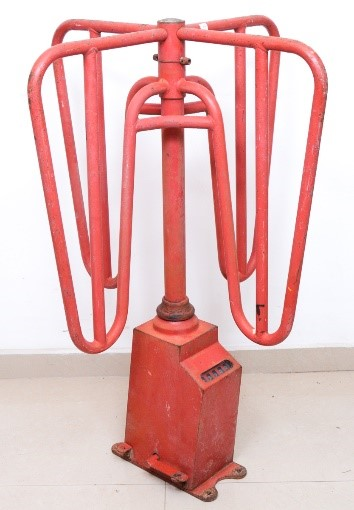
\includegraphics[width=0.95in,height=1.75in]{./media/catraca_antiga.jpg}
	  \caption{Catraca Antiga}
	  \label{fig:older}
	  \source{\cite{antiga}.}
	\end{minipage}%
	\begin{minipage}{.5\textwidth}
		\centering
		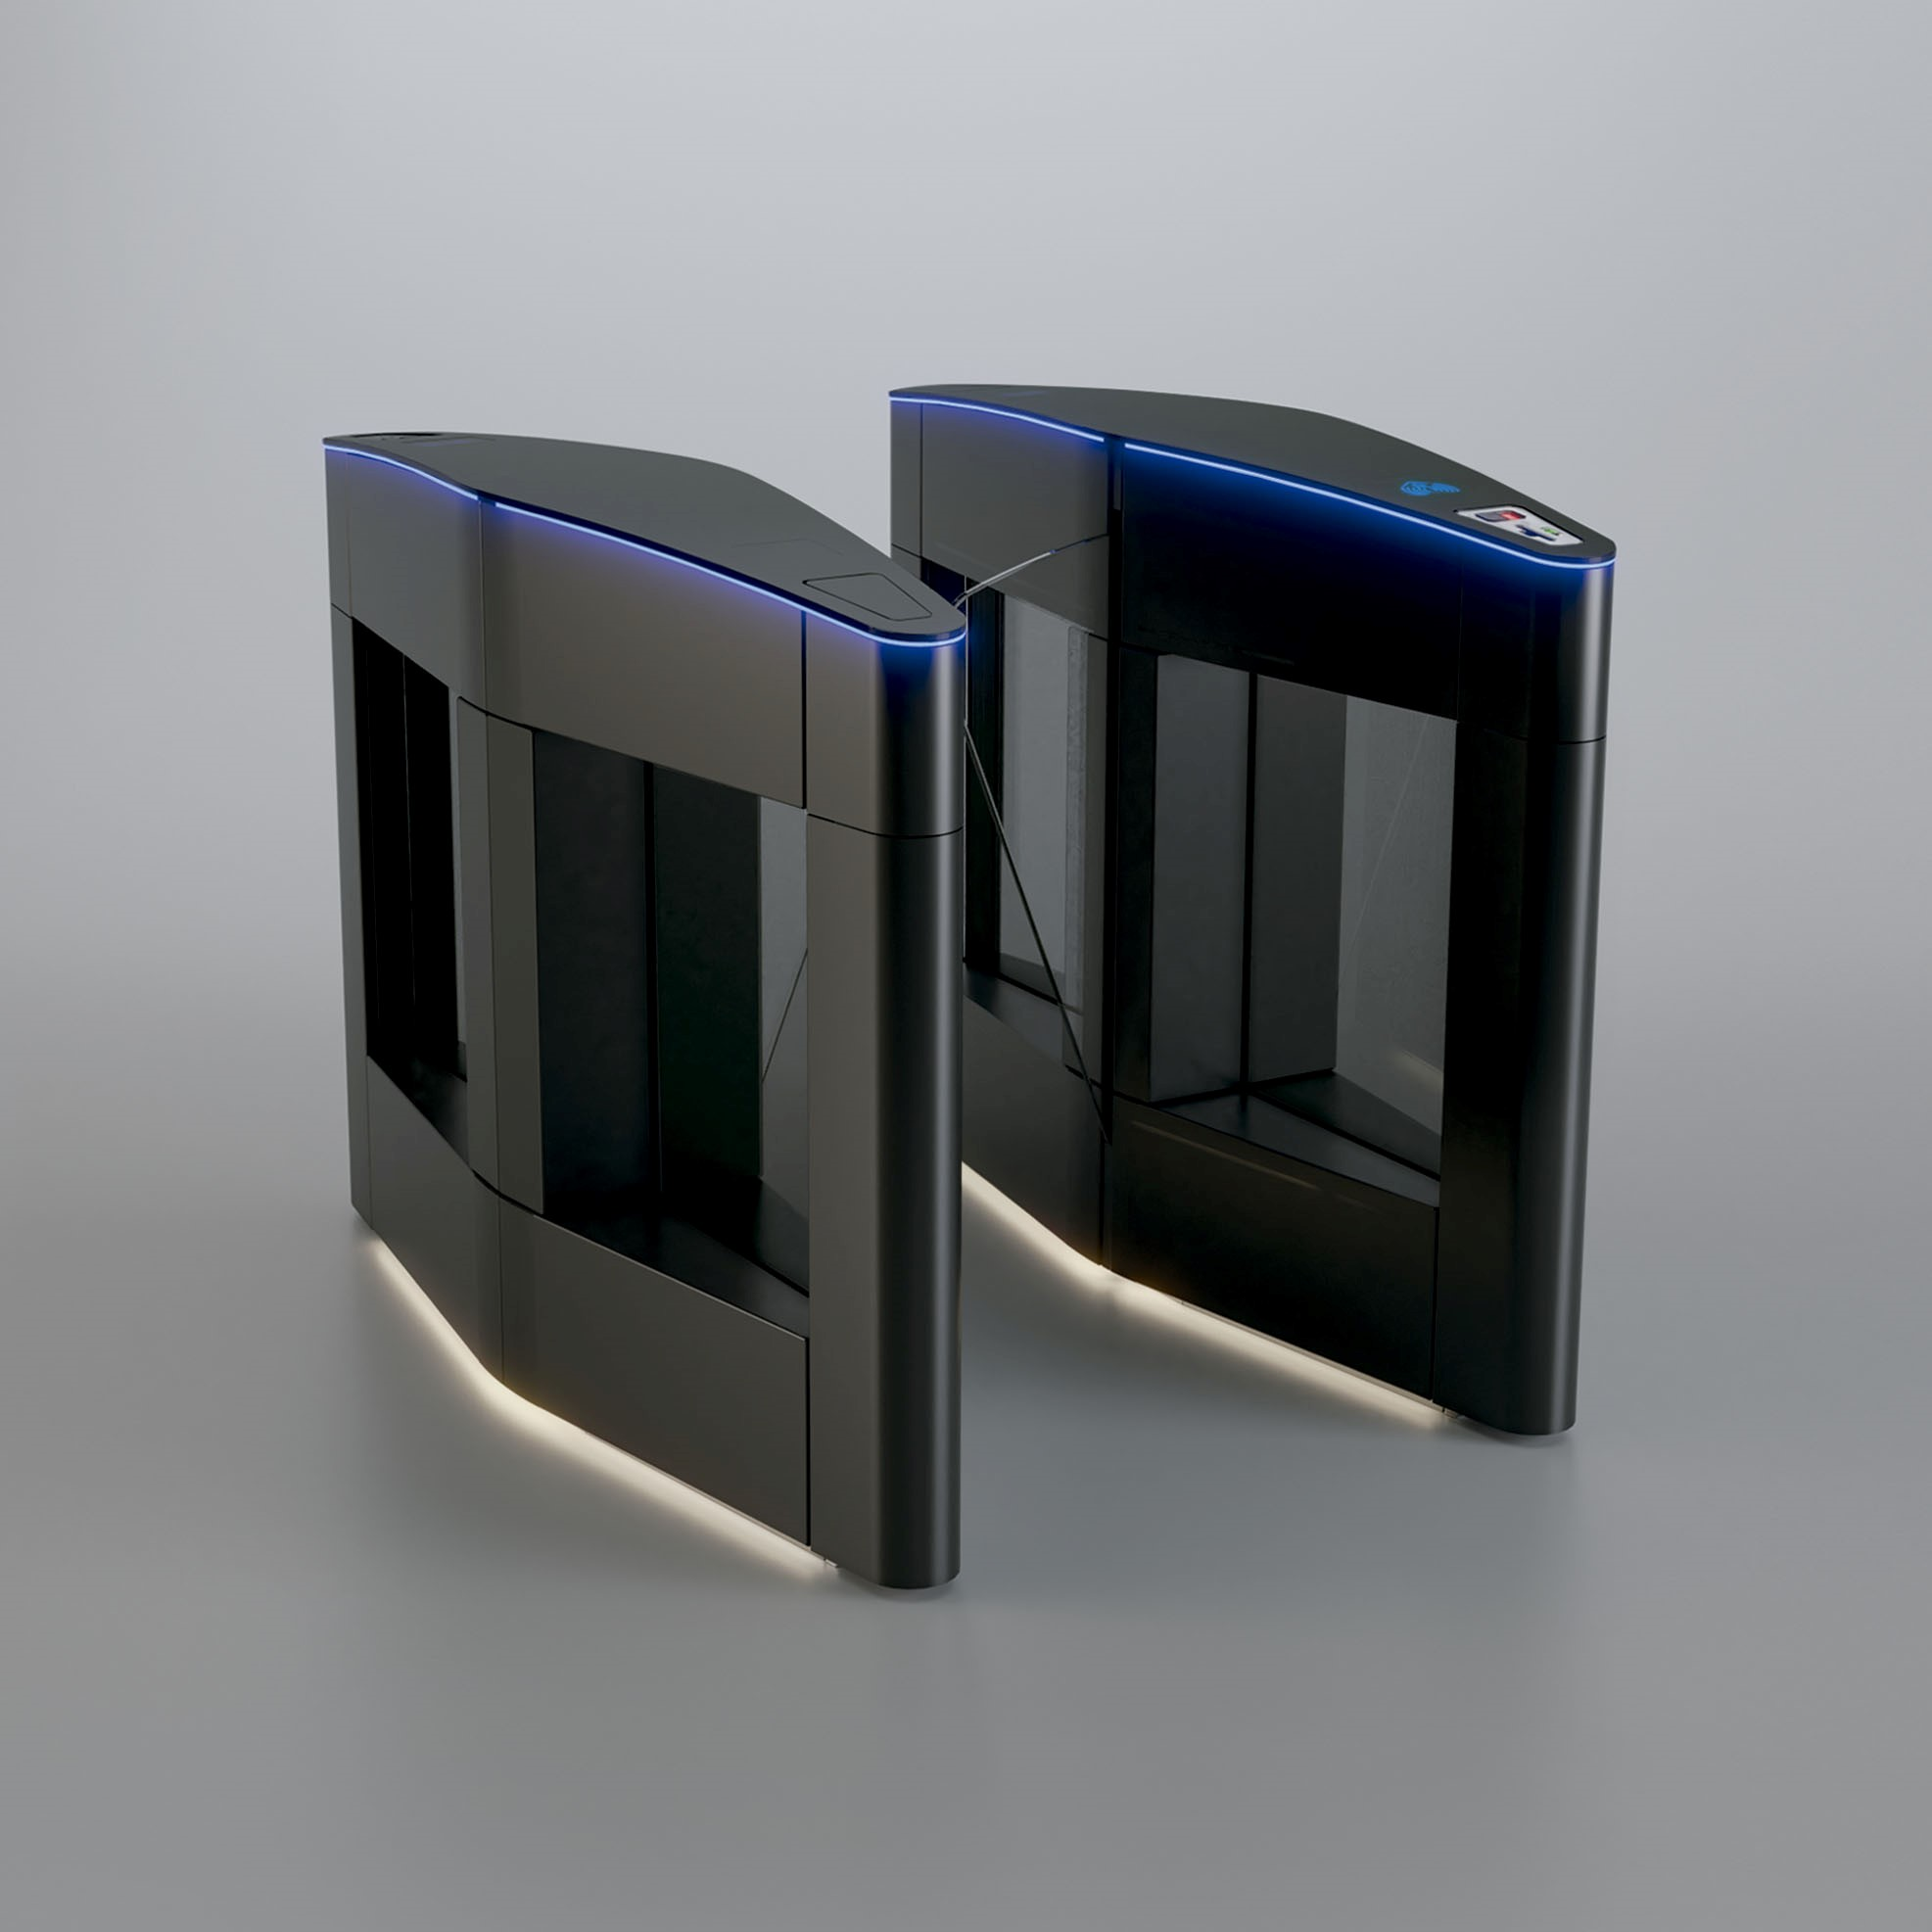
\includegraphics[width=0.95in,height=1.75in]{./media/catraca_nova.jpg}
		\caption{Catraca Nova}
		\label{fig:new}
		\source{\cite{nova}.}
	\end{minipage}
	  \end{figure}

%%%%%%%%%%%%%%%%%%%% Figure/Image No: 6 Ends here %%%%%%%%%%%%%%%%%%%%

\subsection{Internet das Coisas (IoT)}
Tendo seu primeiro uso conhecido sido feito por Kevin Auston, no que diz respeito ao termo IoT, do inglês “Internet of Things”, ou “Internet das Coisas” em tradução livre, temos a união de dois outros termos, “Internet” e “coisas”. O termo “internet” se refere a rede mundial interconectada de computadores que através do protocolo de rede TCP/IP conecta servidores e usuários em todo o globo, tendo cerca de 40\% da população mundial inserida, 7.859.533.912 de seres humanos \cite{populacao} para 4,889,155,643 de usuários \cite{usuarios}. Enquanto isso, o termo “coisas” faz referência a todo e qualquer objeto distinguível no mundo real, eletrônicos ou não, seres vivos ou não. Tendo esclarecido este ponto, não há uma única e verdadeira definição para este termo, no entanto o que a maioria dessas definições tem em comum é a ideia de que se trata de uma rede aberta e compreensível de objetos inteligentes capaz de auto-organizar e compartilhar dados, recursos e informações, reagindo e agindo de acordo com as mudanças no ambiente. Podendo ser considerada uma rede global onde a comunicação entre humanos, humanos e coisas e entre coisas pode ser feita, descrevendo um universo onde tudo pode estar interligado. \cite{iot}

\section{Trabalhos Relacionados}
Este capítulo tem como um dos seus objetivos apresentar e diferenciar os softwares e ferramentas já presentes no mercado, exemplificando suas qualidades e imprecisões e como esses contribuem para o contexto.

\subsection{Relatório Para Aquisição de Novas Catracas}
\subsubsection{Tecnibra}
A Tecnibra é uma empresa localizada no estado de Minas Gerais que utiliza software de terceiros em seus equipamentos, o mesmo permite até 4000 registros e pode trabalhar até com 4 leitores simultâneos: teclado, proximidade RFID, MIFARE, HID e leitor de impressão digital. As catracas oferecidas por essa empresa possuem garantia de 12 meses contra defeitos de fabricação. Tendo orçado em R\$ 8.560,74 cada um dos aparelhos com software de gestão para 8000 usuários.
\subsubsection{Hitech}
A Hitech é uma empresa localizada no estado do Rio de Janeiro, seus equipamentos que possuem
comunicação via RS-232, RS-485 ou TCP/IP com leitura de código de barras,
magnético ou proximidade com leitores independentes para usuário e visitantes,
pictograma orientativo e software DMP Acess II. As catracas oferecidas por essa empresa foram orçadas em R\$ 16.000,00 cada um dos aparelhos e o software de gestão em R\$ 9.000,00, além dos valores da licença do software, treinamento e contrato preventivo.
\subsubsection{Madis}
A Madis é uma empresa localizada no estado de São Paulo, seus equipamentos possuem pictogramas orientativos e direcionais com dois leitores de
proximidade Acura nas extremidades e versão biométrica que comporta 5000
funcionários utilizando somente a biometria 1:N (Só Digital) e 100.000 pessoas no
modo 1:1 (Cartão + Digital), possui capacidade de gerenciamento de até 100.000
usuários (cartões) armazenamento de até 200.000 eventos, o software oferecido é o
MD ACESSO SQL Pontos Ilimitados, No-Break inteligente para até 4 horas e a
memória para armazenamento de dados é SDCARD. As catracas oferecidas por essa empresa possuem garantia de 36 meses contra defeitos de fabricação. Tendo orçado em R\$ 16.593,00 cada um dos aparelhos e o software de gestão em R\$ 10.780,00, além do contrato de manutenção.

Como visto acima, há empresas que ofertam catracas com \textit{softwares}, próprios ou tercerizados, de diversos tipos, com diversos tipos de licenças e garantias. No entanto, o que há de semelhante entre estes produtos é o alto valor ofertado pelo conjunto mesmo que sejam tecnologias diferente, não havendo nenhuma empresa que oferte-os por um preço que, na realidade orçamentária brasileira, possa ser enxergado como baixo e os compradores não possuem qualquer flexibilização ou customização do sistema que irão receber. 

\subsection{Trabalhos Acadêmicos}
\subsubsection{Primeiro Trabalho}
O artigo "SEGURANÇA NAS INSTITUIÇÕES FEDERAIS DE ENSINO:
ESTUDO DE CASO DO IFSC ARARANGUÁ" \cite{sifeecia} apresenta a importância de aumentar a segurança no IF de Santa Catarina, unidade Araranguá, através de sistemas de controle de acesso e como o uso de tecnologia de rádio frequência (RFID) revelou-se uma possiblidade devido suas características e facilidade de uso. Se comparado a esta monografia ambas buscam objetivos semelhantes, no entanto o uso de tecnologia RFID aumenta significativamente o custo, uma vez que para a fabricação de cartões magnéticos compatíveis seria necessário uma quantidade maior de recursos, onde o valor de cada cartão RFID \cite{rfid} equivale a cerca de 5 cartões de PVC convencionais \cite{pvc}. O que fere um dos pontos chave deste trabalho, a economia.
\subsubsection{Segundo Trabalho}
A monografia "PROTÓTIPO DE CONTROLE DE ACESSO UTILIZANDO RFID PARA AUTOMATIZAÇÃO DA SEGURANÇA INTERNA DA UFERSA - CAMPUS MOSSORÓ" \cite{asiufersa} assim como o primeiro trabalho apresenta uma solução para o controle de acesso utilizando RFID. No entanto, aqui o autor mostra como utilizar a automação por meio de placas Arduino \cite{arduino}, que são placas eletrônicas capazes de interagir com o ambiente através de múltiplos sensores, utilizadas principalmente em projetos que tem como objetivo criar "objetos inteligentes" que compartilharão dados e auxiliarão no processamento de informações. Sendo relativamente similar a este projeto, tendo como falha a mesma apresentada no trabalho anterior por utilizar técnicas RFID.

% \chapter{Metodologia}
\label{cap:metodologia}
Este capítulo apresenta as técnicas, tecnologias e ferramentas utilizadas no desenvolvimento da aplicação.

Neste trabalho foi proposto um processo para obtenção de valores mais precisos de \gls{K-IC}, e este segue o seguinte roteiro, conforme o modelo apresentado na \autoref{fig:metodologia_tese}.


\tikzstyle{decision} = [diamond, draw, fill=orange!30, 
    text width=4.5em, text badly centered, node distance=3cm, inner sep=0pt]
\tikzstyle{block} = [rectangle, draw, fill=blue!20, 
    text width=6em, text centered, rounded corners, minimum height=4em]
\tikzstyle{line} = [draw, -latex']
\tikzstyle{cloud} = [draw, ellipse,fill=red!20, node distance=3cm,
    minimum height=2em]

\tikzstyle{startstop} = [rectangle, rounded corners, minimum width=3cm, minimum height=1cm,text centered, draw=black, fill=red!30]
\tikzstyle{process} = [rectangle, minimum width=3cm, minimum height=1cm, text centered, draw=black, fill=blue!20]

\begin{figure}[H]
\centering
\resizebox{!}{15cm} {
\begin{tikzpicture}[node distance = 1.5cm, auto]
    % Place nodes
    \node [startstop] (init) {Determinação de $K_{IC}$};
    %node [block] (init) {determinação de $K_{IC}$};
    \node [process, below of=init] (confeccaoL) {Confecção CPL p/ compressão};
    \node [process, below of=confeccaoL] (compressao) {Ensaio de compressão};
    \node [process, below of=compressao] (propriedades) {Determinação de E e $\nu$};
    \node [process, below of=propriedades] (confeccaoF) {Confecção CP flexão};
    \node [process, below of=confeccaoF] (flexao) {Ensaio de flexão CP liso};
    \node [process, below of=flexao] (kic_preliminar) {Ensaios $K_{IC}$ preliminares};
    \node [process, below of=kic_preliminar] (tdc) {Estimativa $\rho_{min}$ pela TDC};
    \node [decision, below of=tdc, node distance=2.3cm] (decisao) {Comport. Trinca?};
    \node [process, left of=decisao, xshift=-1cm, yshift=-2cm] (gomez) {Aplicar o Critério de Gómez};
    \node [process, right of=decisao, xshift=1cm, yshift=-2cm] (curvaR) {Corrigir com Curva-R};
    \node [process, below of=gomez] (kuc) {$K^{U}_{C}$};
    \node [process, below of=curvaR] (kic) {$K_{IC}$};
    \node [process, below of=kuc] (kicg) {$K_{IC}^{*}$};
    \node [process, below of=kic] (kin_kmax) {$K_{IN},K_{MAX}$};
    \node [startstop, below of=kuc, xshift=2.5cm, yshift=-1.5cm] (stop) {Fim};

    % Draw edges
    \path [line] (init) -- (confeccaoL);
    \path [line] (confeccaoL) -- (compressao);
    \path [line] (compressao) -- (propriedades);
    \path [line] (propriedades) -- (confeccaoF);
    \path [line] (confeccaoF) -- (flexao);
    \path [line] (flexao) -- (kic_preliminar);
    \path [line] (kic_preliminar) -- (tdc);
    \path [line] (tdc) -- (decisao);
    \path [line] (decisao) -- node {não} (gomez); % (gomez)+(-0.3,0.9)
    \path [line] (decisao) -- node {sim} (curvaR);
    \path [line] (gomez)  -- (kuc);
    \path [line] (curvaR) -- (kic);
    \path [line] (kuc)  -- (kicg);
    \path [line] (kic) -- (kin_kmax);
    \path [line] (kicg)  -- (stop);
    \path [line] (kin_kmax) -- (stop);
\end{tikzpicture}
}
\caption{Metodologia para determinação de $K_{Ic}$ desta Tese.}
\label{fig:metodologia_tese}
\end{figure}



\section{Etapas da Pesquisa}


A \glsdesc{a-0} e o \glsdesc{rho}, foram digitados na planilha, visando o cálculo da \glsdesc{K-I}, utilizando a Equações \ref{eq:tenacidade-Tada} e \ref{eq:F-a-h-Tada},

\begin{equation}
\label{eq:tenacidade-Tada}
K_{I} = \sigma_{max} \sqrt{\pi a} \cdot F(a/h)
\; ,
\end{equation}
\begin{equation}
\label{eq:F-a-h-Tada}
\selectlanguage{brazil}
F(a/h) = 1.122 - 1.40 (a/h) + 7.33 (a/h)^{2} - 13.08(a/h)^{3} + 14.0 (a/h)^{4}
\; ,
\end{equation}
\begin{conditions}
$\glssymbol{K-I}$			& \text{\glsdesc{K-I}} \\
$\glssymbol{sigma-max}$		& \text{\glsdesc{sigma-max}} \\
$\glssymbol{a}$				& \text{\glsdesc{a}} \\
$\glssymbol{h}$				& \text{\glsdesc{h}} \\
$\glssymbol{F-a-h}$			& \text{\glsdesc{F-a-h}} \\
\end{conditions}




\section{AAA}

A citação online é utilizada como parte da frase, fazendo sentido na mesma, conforme neste exemplo originalmente citado por \citeonline{kobayashi1999}. Obviamente este autor não tem nada a ver com a frase.

\section{Ferramentas}

Nesta seção é apresentada um exemplo de Tabela (\autoref{tb:weibull_02_09}) adicionada ao texto no formato \LaTeX.



\begin{table}[H]
\centering
\caption{Distribuição de Weibull com a serra de \SI{0.20}{\mm}, $a_{0} \approx \SI{9}{\mm}$}
\label{tb:weibull_02_09}
%\rotatebox{90} {
%\resizebox{!}{7cm} {
\resizebox{14cm}{!} {
\begin{tabular}{@{}rrrrrrrrr@{}}
\toprule
i & \# cp & $sigma_{nom} (MPa)$ & $PF = \dfrac{i - 0.5}{n}$ & $X = ln(\sigma_nom)$ & $Y = ln\left(ln\left(\dfrac{1}{1-Pf}\right)\right)$ & Sxx & Syy & Sxy \\ 
\midrule
1 & 209 & 4.74 & 0.02 & 1.56 & -3.90 & 0.01 & 11.13 & 0.37 \\
2 & 214 & 4.93 & 0.06 & 1.59 & -2.78 & 0.01 & 4.91 & 0.16 \\
3 & 223 & 4.96 & 0.10 & 1.60 & -2.25 & 0.00 & 2.84 & 0.11 \\
4 & 211 & 5.08 & 0.14 & 1.62 & -1.89 & 0.00 & 1.76 & 0.06 \\
5 & 202 & 5.10 & 0.18 & 1.63 & -1.62 & 0.00 & 1.11 & 0.04 \\
6 & 225 & 5.14 & 0.22 & 1.64 & -1.39 & 0.00 & 0.68 & 0.03 \\
7 & 206 & 5.15 & 0.26 & 1.64 & -1.20 & 0.00 & 0.40 & 0.02 \\
8 & 224 & 5.19 & 0.30 & 1.65 & -1.03 & 0.00 & 0.22 & 0.01 \\
9 & 204 & 5.19 & 0.34 & 1.65 & -0.88 & 0.00 & 0.10 & 0.01 \\
10 & 201 & 5.30 & 0.38 & 1.67 & -0.74 & 0.00 & 0.03 & 0.00 \\
11 & 216 & 5.30 & 0.42 & 1.67 & -0.61 & 0.00 & 0.00 & 0.00 \\
12 & 220 & 5.31 & 0.46 & 1.67 & -0.48 & 0.00 & 0.01 & 0.00 \\
13 & 219 & 5.33 & 0.50 & 1.67 & -0.37 & 0.00 & 0.04 & 0.00 \\
14 & 215 & 5.33 & 0.54 & 1.67 & -0.25 & 0.00 & 0.10 & 0.00 \\
15 & 208 & 5.34 & 0.58 & 1.67 & -0.14 & 0.00 & 0.18 & 0.00 \\
16 & 203 & 5.35 & 0.62 & 1.68 & -0.03 & 0.00 & 0.28 & 0.00 \\
17 & 222 & 5.43 & 0.66 & 1.69 & 0.08 & 0.00 & 0.41 & 0.02 \\
18 & 207 & 5.48 & 0.70 & 1.70 & 0.19 & 0.00 & 0.56 & 0.02 \\
19 & 213 & 5.51 & 0.74 & 1.71 & 0.30 & 0.00 & 0.75 & 0.03 \\
20 & 205 & 5.52 & 0.78 & 1.71 & 0.41 & 0.00 & 0.96 & 0.04 \\
21 & 221 & 5.54 & 0.82 & 1.71 & 0.54 & 0.00 & 1.22 & 0.05 \\
22 & 210 & 5.55 & 0.86 & 1.71 & 0.68 & 0.00 & 1.54 & 0.06 \\
23 & 217 & 5.56 & 0.90 & 1.72 & 0.83 & 0.00 & 1.96 & 0.07 \\
24 & 218 & 5.61 & 0.94 & 1.73 & 1.03 & 0.00 & 2.56 & 0.09 \\
25 & 212 & 5.75 & 0.98 & 1.75 & 1.36 & 0.01 & 3.72 & 0.16 \\
N = & 25 &  & Médias & 1.67 & -0.57 &  &  &  \\
 &  &  &  &  & Somas & 0.05 & 37.48 & 1.35 \\ 
\bottomrule
\end{tabular}
}
%}
\end{table}

Outro exemplo importante é o de Tabelas em LandScape, conforme a \autoref{tb:dados_cp_flexao_02_09}

Estudos envolvendo física, engenharia e matemática em geral precisam utilizar letras gregas. Tais letras podem ser utilizados dentro de equações matemáticas no \LaTeX. Quando for necessário utilizá-las em frases comuns deve-se utilizar o recurso de expressão em linha, adicionando um cifrão antes e outro depois da expressão criada, como em $\alpha , \beta , \delta, \gamma $ ...

% \chapter{DESENVOLVIMENTO}
\label{cap:desenvolvimento}
Vestibulum ac arcu suscipit, consequat orci sit amet, maximus dolor. Vestibulum condimentum nulla vitae fermentum venenatis. In sit amet tincidunt ex, quis molestie turpis. Proin eleifend fringilla tincidunt. Curabitur pellentesque nisi in risus iaculis, in tristique odio maximus. Donec condimentum massa a erat malesuada, ut lacinia elit maximus. Integer feugiat volutpat luctus. Vestibulum commodo varius venenatis. Ut diam ante, feugiat non consectetur id, suscipit at dolor. Duis tempor quam ligula, id volutpat ligula dapibus id. Phasellus at fermentum nibh.

\section{Levantamento das Estórias}

As estórias foram identificadas, analisadas e descritas abaixo:

\begin{itemize}
	\item \textbf{Estória 01: Cadastrar Catador}\par
Descrição: Permite a criação do usuário responsável pelo recolhimento do material descartado.

	\item \textbf{Estória 02: Cadastrar Separador}\par
Descrição: Permite a criação do usuário responsável pelo descarte do material.

	\item \textbf{Estória 03: Efetuar login}\par
Descrição: Autoriza o acesso às funcionalidades do sistema. 

	\item \textbf{Estória 04: Recuperar senha }\par
Descrição: Possibilita que o usuário redefina a senha.

	\item \textbf{Estória 05: Tirar dúvidas }\par
Descrição: Esclarece sobre a definição dos perfis. 

	\item \textbf{Estória 06: Solicitar recolhimento}\par
Descrição: Requisita a coleta do material descartado.

	\item \textbf{Estória 07: Realizar logoff}\par
Descrição: Permite que o usuário saia do sistema.

\end{itemize}


\section{Diagramas do Modelo Proposto}

\subsection{Diagrama de Classes}

Na construção do diagrama de classes foi analisada as principais classes do sistema, suas características, seus relacionamentos e suas funcionalidades. É possível observar através da \autoref{fig:classe}, a estrutura do desenvolvimento do sistema.

%%%%%%%%%%%%%%%%%%%% Figure/Image No: 8 starts here %%%%%%%%%%%%%%%%%%%%

\begin{figure}[H]
	\begin{Center}
		\includegraphics[width=6.4in,height=2.77in]{./media/image35.png}
	\end{Center}
	\caption{Diagrama de Classes}
	\label{fig:classe}
\end{figure}

%%%%%%%%%%%%%%%%%%%% Figure/Image No: 8 Ends here %%%%%%%%%%%%%%%%%%%%

Na \autoref{fig:classe} citada acima podemos observar o Diagrama de Classes utilizado para a construção do aplicativo.

As classes Catador e Separador são extensões da classe Pessoa, que tem como objetivo informar seus dados, tirar dúvidas sobre a definição dos perfis, criar uma conta perfil, redefinir a senha esquecida, efetuar \textit{login}, salvar os dados do \textit{login} e realizar \textit{logoff}.

A classe Catador que faz parte de uma das contas perfil, é responsável pelo cadastro do usuário catador. Este usuário é encarregado por traçar a rota da coleta e recolher o material descartado.

A classe Separador que faz parte de uma das contas perfil, é responsável pelo cadastro do usuário separador. Ao informar sua localização e o tipo de material, o usuário poderá solicitar o recolhimento do material descartado.

\subsection{Diagrama de Casos de Uso}

Esse parágrafo descreve as funcionalidades do sistema e as interações entre os atores, através da \autoref{fig:casos}. 

%%%%%%%%%%%%%%%%%%%% Figure/Image No: 9 starts here %%%%%%%%%%%%%%%%%%%%

\begin{figure}[H]
	\begin{Center}
		\includegraphics[width=5.12in,height=3.02in]{./media/image32.png}
	\end{Center}
	\caption{Diagrama de Casos de Uso}
	\label{fig:casos}
\end{figure}

%%%%%%%%%%%%%%%%%%%% Figure/Image No: 9 Ends here %%%%%%%%%%%%%%%%%%%%

Na \autoref{fig:casos} citada acima, podemos ver o Diagrama de Casos de Uso. Na tela inicial do aplicativo, o usuário poderá realizar as seguintes funções: logar no APP, cadastrar usuário, tirar dúvidas, efetuar \textit{logoff} e recuperar a senha. Se o usuário ainda não estiver cadastrado, irá se cadastrar no perfil desejado: Catador ou Separador. Caso já tenha cadastro, basta efetuar o \textit{login}, o qual pode ser salvo pelo sistema. Em caso de senha esquecida, o sistema permite a recuperação através do \textit{e-mail}.

A partir da inserção da localização e do tipo de material, o Separador poderá solicitar o recolhimento do rejeito. O Catador recebendo a solicitação do Separador, irá traçar a rota para a coleta do material. 

\paragraph*{5.2.2.1 Especificação dos Casos de Uso}

Esse capítulo é responsável pelo detalhamento das funcionalidades do sistema. O (\autoref{quad:catador}), descreve o passo a passo para o cadastro do usuário Catador.

%%%%%%%%%%%%%%%%%%%% Table No: 4 starts here %%%%%%%%%%%%%%%%%%%%

\begin{quadro}[H]
\caption{Cadastrar Catador}
\label{quad:catador}
\centering
\begin{tabular}{p{1.25in}p{4.50in}}
\hline
%row no:1
\multicolumn{1}{|p{1.25in}}{\textbf{Caso de Uso}} & 
\multicolumn{1}{|p{4.50in}|}{Cadastrar Catador} \\
\hhline{--}
%row no:2
\multicolumn{1}{|p{1.25in}}{\textbf{Descrição}} & 
\multicolumn{1}{|p{4.50in}|}{Permite a criação de perfil usuário denominado catador.} \\
\hhline{--}
%row no:3
\multicolumn{1}{|p{1.25in}}{\textbf{Ator}} & 
\multicolumn{1}{|p{4.50in}|}{Catador} \\
\hhline{--}
%row no:4
\multicolumn{1}{|p{1.25in}}{\textbf{Pré-condições}} & 
\multicolumn{1}{|p{4.50in}|}{Preencher todos os dados solicitados} \\
\hhline{--}
%row no:5
\multicolumn{1}{|p{1.25in}}{\textbf{Pós-condições}} & 
\multicolumn{1}{|p{4.50in}|}{Cadastro do perfil catador no sistema} \\
\hhline{--}
%row no:6
\multicolumn{1}{|p{1.25in}}{\textbf{Fluxo Principal}} & 
\multicolumn{1}{|p{4.50in}|}{\begin{enumerate}[label*={\fontsize{12pt}{12pt}\selectfont \arabic*.}]
	\item Na tela inicial, o usuário solicita o cadastro; \par 	\item Em seguida preenche todos os dados; \par 	\item O sistema valida os dados preenchidos; \par 	\item O cadastro é realizado.
\end{enumerate}} \\
\hhline{--}
%row no:7
\multicolumn{1}{|p{1.25in}}{\textbf{Fluxo de Exceção}} & 
\multicolumn{1}{|p{4.50in}|}{\textbf{Dados incorretos} \par \begin{enumerate}[label*={\fontsize{12pt}{12pt}\selectfont \arabic*.}]
	\item No passo 3 do Fluxo Principal, o usuário não preencheu os dados corretamente, o sistema sinaliza qual campo não foi preenchido.
\end{enumerate} \par \textbf{Dados não cadastrados} \par \begin{enumerate}[label*={\fontsize{12pt}{12pt}\selectfont \arabic*.}]
	\item No passo 3 do Fluxo Principal, o usuário preenche algum campo já cadastrado, o sistema exibe qual campo já foi cadastrado.
\end{enumerate}} \\
\hhline{--}

\end{tabular}
\end{quadro}


%%%%%%%%%%%%%%%%%%%% Table No: 4 ends here %%%%%%%%%%%%%%%%%%%%

O caso de uso Cadastrar Catador (\autoref{quad:catador}), citado acima é responsável por avaliar as ações necessárias para realizar o cadastro do perfil catador. 

O \autoref{qua:separador} descreve o passo a passo para o cadastro do usuário Separador.

%%%%%%%%%%%%%%%%%%%% Table No: 5 starts here %%%%%%%%%%%%%%%%%%%%


\begin{quadro}[H]
\caption{Cadastro Separador}
 \label{qua:separador}			\begin{tabular}{p{1.33in}p{3.96in}}
\hline
%row no:1
\multicolumn{1}{|p{1.33in}}{\textbf{Caso de Uso}} & 
\multicolumn{1}{|p{3.96in}|}{Cadastrar Separador} \\
\hhline{--}
%row no:2
\multicolumn{1}{|p{1.33in}}{\textbf{Descrição}} & 
\multicolumn{1}{|p{3.96in}|}{Permite a criação de perfil usuário denominado separador.} \\
\hhline{--}
%row no:3
\multicolumn{1}{|p{1.33in}}{\textbf{Ator}} & 
\multicolumn{1}{|p{3.96in}|}{Separador} \\
\hhline{--}
%row no:4
\multicolumn{1}{|p{1.33in}}{\textbf{Pré-condições}} & 
\multicolumn{1}{|p{3.96in}|}{Preencher todos os dados solicitados } \\
\hhline{--}
%row no:5
\multicolumn{1}{|p{1.33in}}{\textbf{Pós-condições}} & 
\multicolumn{1}{|p{3.96in}|}{Cadastro do perfil separador no sistema} \\
\hhline{--}
%row no:6
\multicolumn{1}{|p{1.33in}}{\textbf{Fluxo Principal}} & 
\multicolumn{1}{|p{3.96in}|}{\begin{enumerate}[label*={\fontsize{12pt}{12pt}\selectfont \arabic*.}]
	\item Na tela inicial, o usuário solicita o cadastro; \par 	\item Em seguida, preenche todos os dados; \par 	\item O sistema verifica os dados; \par 	\item O cadastro é realizado.
\end{enumerate}} \\
\hhline{--}

\end{tabular}
 \end{quadro}

%%%%%%%%%%%%%%%%%%%% Table No: 5 ends here %%%%%%%%%%%%%%%%%%%%

O caso de uso Cadastrar Separador (\autoref{qua:separador}), citado acima é responsável por avaliar as ações necessárias para realizar o cadastro do perfil separador.





% 
\chapter{RESULTADOS E DISCUSSÕES}
%%%%%%%%%%%%%%%%%ALTERADO%%% %%%%%%%%%%%%%%%%%%%%
\label{cap:resultados}
 Neste capítulo são apresentados os resultados obtidos após o desenvolvimento do protótipo e a análise dessas informações. O desenvolvimento deste projeto cumpriu as etapas planejadas e teve como resultado um protótipo com dois perfis: O perfil catador, o qual é responsável pelo recolhimento do material e o perfil separador, que solicita o serviço da coleta de resíduos sólidos.

No final do testes foi coletado o questionário de avaliação dos participantes com os itens avaliados, sendo estas informações representadas na \autoref{fig:resultados}.

\begin{figure}[H]
	\begin{Center}
		\includegraphics[width=5.0in,height=3.06in]{./media/resultados.png}
	\end{Center}
\caption{Gráfico dos resultados obtidos do questionário}
\label{fig:resultados}
\end{figure}

Na \autoref{fig:resultados} citada acima foi possível observar que foram criados quatro perfis de usuário: dois perfis separadores e dois perfis catadores. A média dos resultados das perguntas foi satisfatória.

O \autoref{cod:cadbanc0} é responsável por salvar o usuário catador no \textit{firebase realtime database}. A linha 3 do \autoref{cod:cadbanc0}, consiste na criação do nó (\textit{child}) denominado “Catadores”, onde cada catador possui um identificador (\textit{id}), onde seus dados são salvos (\textit{setValue}).

\begin{codigo}[H]
\begin{lstlisting}[language=Java]
public void salvar(){
    DatabaseReference databaseReference = ConfiguracaoFirebase.getFirebase();
    databaseReference.child("Catadores").child(getId()).setValue(this);
}
\end{lstlisting}
\caption{Salvar usuário catador no banco de dados}
\label{cod:cadbanc0}
\end{codigo}


Na \autoref{fig:login} a seguir, é apresentada a tela inicial da aplicação. 
%%%%%%%%%%%%%%%%%%%% Figure/Image No: 54 starts here %%%%%%%%%%%%%%%%%%%%

\begin{figure}[H]
	\begin{Center}
		\includegraphics[width=1.85in,height=2.94in]{./media/image34.png}
	\end{Center}
\caption{Tela de Login}
\label{fig:login}
\end{figure}
%%%%%%%%%%%%%%%%%%%% Figure/Image No: 54 Ends here %%%%%%%%%%%%%%%%%%%%
Na tela inicial (\autoref{fig:login}) da aplicação citada acima, o usuário já cadastrado irá informar seu \textit{e-mail} e senha e realizar o \textit{login} no sistema. A aplicação permite a visualização da senha digitada e o armazenamento dos dados de autenticação.


% \chapter{Conclusão}
\label{cap:conclusão}
%%%%%%%%%%%ALTERADO%%%%%%%
Orci varius natoque penatibus et magnis dis parturient montes, nascetur ridiculus mus. Aenean nec pulvinar libero, et pellentesque elit. Sed a congue sapien. Etiam pretium ligula sit amet blandit porttitor. Cras accumsan pretium eros ut imperdiet. Donec vel lacus ante. Quisque consectetur ligula sit amet leo accumsan lobortis gravida sit amet lacus. Integer a leo nisl. Mauris pretium fringilla lobortis. Ut condimentum, lorem vitae viverra tincidunt, est mauris ornare augue, ac semper mi lorem et enim. Vestibulum venenatis id sapien vel volutpat. Pellentesque ut porta nisi. Pellentesque mattis metus a quam congue, sit amet viverra ex auctor.

Além disso, com a informação do tipo de material depositado pelo separador, o catador otimiza seu tempo, podendo ter um maior número de materiais recolhidos, e com a facilidade de escolher onde descartar o material separado, mais pessoas podem realizar a separação de materiais em suas rotinas. 

Class aptent taciti sociosqu ad litora torquent per conubia nostra, per inceptos himenaeos. Morbi pretium posuere augue nec varius. Sed ac sem in magna dapibus iaculis. Nam elementum neque eget tellus viverra scelerisque. Aenean ut posuere elit. Morbi eget erat non ante congue tempor eget id erat. Nulla quis luctus nulla. Mauris auctor vel magna sed ultrices. Integer in massa molestie, ornare urna id, viverra sem. Vivamus interdum, ligula eget convallis tempor, dui tellus tristique nibh, in interdum arcu sem a tellus. 

\section{Trabalhos Futuros}

Maecenas id nisi vel neque tincidunt faucibus quis at nibh. Aenean consequat eleifend ultrices. Cras dui nibh, luctus a nibh ultrices, condimentum gravida diam. Cras dapibus sit amet mauris at pharetra. Vestibulum quis malesuada mi. Nunc pretium, neque at placerat maximus, urna nunc hendrerit urna, eget efficitur sem ipsum vel mauris. Donec eget efficitur eros, at cursus dolor.

\begin{itemize}
	\item Acrescentar todos os pontos de descarte no mapa;
	\item Otimizar a rota através de algoritmos;
	\item Aplicar filtros ao mapa, para que o catador possa visualizar somente os pontos pelo tipo de material selecionado;
	\item Enviar notificações quando forem inseridos novos pontos de descarte e quando for sinalizado o recolhimento de um material;
\setlength{\parskip}{9.96pt}
	\item Adicionar outros métodos de \textit{login}, como por exemplo: o \textit{Facebook, }o \textit{Gmail }e o número de telefone;
	\item Inserir uma rota dinâmica no programa, em função da localização instantânea do usuário.
\end{itemize}

 \glsaddall

% \postextual

\bibliography{Referencias}

% Imprime uma página indicando o início dos apêndices
% \partapendices
% \part*{Apêndices}

% \begin{apendicesenv}

% 
\chapter{Questionário de Avaliação do Protótipo}

\begin{figure}[H]
	\begin{Center}
		\includegraphics[width=6.00in]{media/questionariopaint.png}
		\label{fig:questionario}
	\end{Center}
\end{figure}

\chapter{Códigos fonte comentados}

\section{Salvar usuário catador no banco de dados}

O \autoref{cod:cadbanc} é responsável por salvar o usuário catador no \textit{firebase realtime database}. A linha 3 do \autoref{cod:cadbanc}, consiste na criação do nó (\textit{child}) denominado “Catadores”, onde cada catador possui um identificador (\textit{id}), onde seus dados são salvos (\textit{setValue}).

\begin{codigo}[H]
\begin{lstlisting}[language=Java]
public void salvar(){
    DatabaseReference databaseReference = ConfiguracaoFirebase.getFirebase();
    databaseReference.child("Catadores").child(getId()).setValue(this);
}
\end{lstlisting}
\caption{Salvar usuário catador no banco de dados}
\label{cod:cadbanc}
\end{codigo}


\section{Salvar usuário separador no banco de dados}

\begin{codigo}[H]
	\begin{lstlisting}[language=Java]
public void salvar(){
    DatabaseReference databaseReference = ConfiguracaoFirebase.getFirebase();
    databaseReference.child("Separadores").child(getId()).setValue(this);
}
   	\end{lstlisting}
   	\caption{Salvar usuário separador no banco de dados}
   	\label{cod:cadsep}
\end{codigo}

O \autoref{cod:cadsep} é responsável por salvar o usuário separador no \textit{firebase realtime database}. A linha 3 do \autoref{cod:cadbanc}, consiste na criação do nó (\textit{child}) denominado “Separadores”, onde cada separador possui um identificador (\textit{id}), onde seus dados são salvos (\textit{setValue}).


\section{Cadastrar usuário catador}

\begin{codigo}[H]
	\begin{lstlisting}[language=Java]
private void cadastrarCatador(){
    firebaseAuth = ConfiguracaoFirebase.getFirebaseAuth();
    firebaseAuth.createUserWithEmailAndPassword(
            catador.getEmail(),
            catador.getSenha()
    ).addOnCompleteListener(CadastroCatador.this, new OnCompleteListener<AuthResult>() {
        @Override
        public void onComplete(@NonNull Task<AuthResult> task) {
            if(task.isSuccessful()){
                Toast.makeText(CadastroCatador.this,"Sucesso ao cadastrar catador",Toast.LENGTH_LONG).show();
                FirebaseUser firebaseUser = task.getResult().getUser();
                catador.setId(firebaseUser.getUid());
                catador.salvar();
                startActivity(new Intent(CadastroCatador.this, Login.class));
       	\end{lstlisting}
       	\caption{Cadastrar usuário catador na aplicação}
       	\label{cod:cat}
\end{codigo}

O \autoref{cod:cat} consiste no cadastro do usuário catador. A função \textit{createUserWithEmailAndPassword}, que se encontra na linha 3, é responsável pela criação da autenticação dos usuário através do \textit{e-mail} e a senha. Em caso de sucesso, o sistema irá exibir a seguinte mensagem “Sucesso ao cadastrar catador” e o usuário será redirecionado para a tela de \textit{login}.

\section{Cadastrar usuário separador}

\begin{codigo}[H]
	\begin{lstlisting}[language=Java]
private void cadastrarSeparador(){
    firebaseAuth = ConfiguracaoFirebase.getFirebaseAuth();
    firebaseAuth.createUserWithEmailAndPassword(
            separador.getEmail(),
            separador.getSenha()
    ).addOnCompleteListener(CadastroSeparador.this, new OnCompleteListener<AuthResult>() {
        @Override
        public void onComplete(@NonNull Task<AuthResult> task) {
            if(task.isSuccessful()){
                Toast.makeText(CadastroSeparador.this,"Sucesso ao cadastrar separador",Toast.LENGTH_LONG).show();
                FirebaseUser firebaseUser = task.getResult().getUser();
                separador.setId(firebaseUser.getUid());
                separador.salvar();
                startActivity(new Intent(CadastroSeparador.this, Login.class));
       	\end{lstlisting}
       	\caption{Cadastrar usuário separador}
       	\label{cod:sep}
\end{codigo}

O \autoref{cod:sep} consiste no cadastro do usuário separador. A função \textit{createUserWithEmailAndPassword}, que se encontra na linha 3, é responsável pela criação da autenticação do usuário através do \textit{e-mail} e a senha.

% \end{apendicesenv}

% \begin{anexosenv}

% 


% \end{anexosenv}

\end{document}
